\section{Simulación}\label{sec:simulacion}

\begin{frame}{Parámetros del sistema}
    \begin{block}{Parámetros fijos}
        \begin{itemize}
            \item Cantidad de partículas - $N = 100$
            \item Masa de la partícula - $m = 0.001\ kg$
            \item Tiempo de simulación - $tf = 300\ s$
            \item Longitud de los resortes - $l = 0.001\ m$
            \item Amplitud de oscilación de la partícula N - $A = 0.01\ m$
        \end{itemize}
    \end{block}
    \begin{block}{Parámetros variables}
        \begin{itemize}
            \item Frecuencia de oscilación de la partícula N - $\omega\ (1/s)$
            \item Constante elástica de los resortes - $k\ (kg/s^2)$
            \item Paso temporal de simulación - $dt\ (s)$
        \end{itemize}
    \end{block}
\end{frame}

\begin{frame}{Esquema del sistema}
    \text{Esquema simplificado con las variables de simulación.}
    \begin{figure}[H]
        \centering
        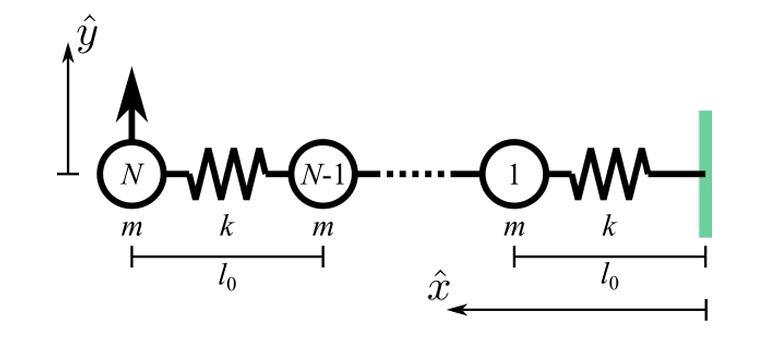
\includegraphics[width=0.8\linewidth]{pic/04-sim/system-schema}\label{fig:figure-system-schema}
    \end{figure}
\end{frame}

\begin{frame}{Observables}
    \begin{block}{Amplitud de oscilación del sistema}
        \text{La máxima amplitud que alcanza cualquier partícula del sistema en un instante de tiempo.}
        \begin{equation*}
            H(t) = \max \left\{\ y_i(t) : 1 \leq i \leq N\ \right\}
        \end{equation*}
    \end{block}

    \begin{block}{Máxima amplitud de oscilación del sistema}
        \text{La máxima amplitud de oscilación alcanzada por el sistema, dada una frecuencia angular.}
        \begin{equation*}
            H_{max}(\omega) = \max \left\{\ H(t) : 0 \leq t \leq tf\ \right\}
        \end{equation*}
    \end{block}
\end{frame}

\begin{frame}{Observables}
    \small{
    \begin{block}{Frecuencia de resonancia}
        \text{Frecuencia angular en la que el sistema alcanza la máxima amplitud de oscilación.}
        \begin{equation*}
            \omega_{0} = \omega\ :\ H_{max}(\omega) \geq H_{max}(\omega_2),\ \forall\omega_2
        \end{equation*}
    \end{block}

    \begin{block}{Relación entre la frecuencia de resonancia y la constante elástica}
        \text{Relación lineal entre la frecuencia de resonancia y la raíz cuadrada de la constante elástica.}
        \begin{equation*}
            \omega_{0}\ \propto \sqrt{k}
        \end{equation*}
    \end{block}

    \begin{block}{Fórmula de error}
        \text{Utilizado para ajustar el factor de proporcionalidad entre $\omega_0$ y $k$.}
        \begin{equation*}
            E(c) = \sum (y_i - f(x_i, c))^2
        \end{equation*}
    \end{block}
    }
\end{frame}

